\documentclass[11pt,a4paper]{article}
\usepackage[utf8]{inputenc}
\usepackage[margin=2.5cm]{geometry}
\usepackage{times}
\usepackage{latexsym}
\usepackage{amsmath,amssymb}
\usepackage{booktabs}
\usepackage{graphicx}
\usepackage{hyperref}
\usepackage{microtype}
\usepackage{tikz}
\usetikzlibrary{arrows.meta,positioning}
% images produced by the pipeline live in ../data_report/ (see scripts/analyze.py)
\graphicspath{{../data_report/}{./}}
\newcommand\BibTeX{B\textsc{ib}\TeX}

\title{FeDAPT: Federated Domain-Adaptive Pre-Training for\\Cross-Domain Security Assistant LLMs}
\author{Damian Villarreal \\
  Summer 2026 GRA Research \\}
\date{\today}

\begin{document}
\maketitle

\begin{abstract}
Large Language Models (LLMs) show immense promise as specialized automated assistants in Security Operations Centers (SOCs). However, training an effective security assistant requires grounding in diverse, multi-domain telemetry (endpoint, network, cloud), which security organizations cannot pool or share due to strict privacy, compliance, and competitive risks. We introduce \textbf{FeDAPT}, a two-stage federated framework designed to collaboratively pre-train a domain-adapted security LLM across a network of organizations without exposing raw, sensitive telemetry. FeDAPT decouples learning into two stages: (1) \emph{Federated Domain-Adaptive Pre-Training (DAPT)} over a shared, public prose corpus (threat intelligence, MITRE ATT\&CK procedures, Sigma rules, CVEs) to learn foundational security language and reasoning, followed by (2) \emph{Local Task Tuning} on private, organization-specific log-to-prose task pairs. We instantiate the framework under non-IID domain skew ($\alpha{=}0.5$), user-level Differential Privacy (DP-FedAvg with RDP accounting), and Byzantine adversarial attacks (sign-flipping, scaling, Gaussian noise, data poisoning), and design a multi-tiered evaluation harness featuring a CLEV-style, reference-aware LLM-as-a-judge validated against human annotations. This paper contributes the framework, the reproducible data pipeline realized to date, and the evaluation methodology; a full empirical evaluation across these settings is ongoing and its experimental design is reported here. Throughout, public datasets are used as a controlled \emph{stand-in} to simulate a private federated setting.
\end{abstract}

\section{Introduction}
Modern Security Operations Centers (SOCs) are overwhelmed by the velocity and heterogeneity of security telemetry. Analysts must rapidly correlate evidence across disparate operational domains---endpoint process trees (Sysmon), network traffic (Zeek, NetFlow, Suricata), and cloud audit trails (AWS CloudTrail, Azure, Okta). While Large Language Models (LLMs) have emerged as powerful tools for automated explanation and triage, deploying off-the-shelf general-purpose LLMs in specialized security environments presents two major challenges:
\begin{enumerate}
    \item \textbf{Domain Specialization vs.\ Privacy Constraints:} A single organization rarely possesses sufficient volume or domain variety in its local telemetry to train a comprehensive security assistant. Yet directly pooling raw telemetry across organizations to train a centralized model conflicts with regulatory mandates (e.g., GDPR, HIPAA), customer privacy contracts, and proprietary boundaries.
    \item \textbf{Telemetry Grounding vs.\ Language Reasoning:} Raw log entries (e.g., JSON blobs or Sysmon XML lines) lack natural-language context. An effective security assistant must bridge the gap between technical log artifacts and human-understandable prose explanations.
\end{enumerate}

To address these challenges, we present \textbf{FeDAPT} (\textbf{Fe}derated \textbf{D}omain-\textbf{A}daptive \textbf{P}re-\textbf{T}raining), a framework designed to answer a fundamental research question: \emph{Can a network of security organizations collaboratively pre-train a superior domain-assistant LLM without sharing their private data?}

FeDAPT establishes a strict, principled separation between shared knowledge and local data:
\begin{itemize}
    \item \textbf{Shared Knowledge Substrate (Prose Corpus):} Public, shareable natural-language security texts (MITRE ATT\&CK, Sigma detection rules, NVD CVE descriptions, CISA KEV) are federated in Stage~1 to pre-train a shared Low-Rank Adaptation (LoRA) domain adapter across organizations.
    \item \textbf{Private Grounding Data (Log Telemetry):} Sensitive log streams remain strictly local to each organization. In Stage~2, clients warm-start from the federated adapter and perform local completion-only task tuning on their own data. In our experiments, public telemetry (\texttt{splunk/attack\_data}) is partitioned across simulated organizations to \emph{stand in} for genuinely private data.
\end{itemize}

\paragraph{Main Contributions.}
\begin{enumerate}
    \item \textbf{Two-Stage Decoupled Architecture:} A clean separation between federated domain-adaptive pre-training on public prose and local completion-only task tuning on private telemetry.
    \item \textbf{Controlled Ablation Framework:} An $A/B/C/D$ ablation matrix (No DAPT, Local DAPT, Federated DAPT, Centralized DAPT) that explicitly isolates the net utility gained by participating in the federated network ($C-B$).
    \item \textbf{Robustness \& Privacy Design:} An instantiation under non-IID Dirichlet skew ($\alpha{=}0.5$), user-level Differential Privacy (RDP-accounted DP-FedAvg), and Byzantine adversary simulations (sign-flip, scaling, noise, data poisoning) across robust aggregators (Krum, Trimmed-Mean).
    \item \textbf{Defensible CLEV Evaluation:} A reference-aware, 2+1 tie-breaking LLM-as-a-judge harness, validated against human annotations via Cohen's $\kappa$ and Macro-$F_1$.
\end{enumerate}

\section{Related Work}
\paragraph{Domain-Adaptive Pre-Training.} Continued pre-training on in-domain text (DAPT) reliably improves downstream task performance in specialized domains~\cite{gururangan2020dapt}. We apply this idea in a \emph{federated} setting and on a security-specific prose corpus.

\paragraph{Federated Learning and LLMs.} FedAvg~\cite{mcmahan2017fedavg} established communication-efficient federated optimization; FedProx~\cite{li2020fedprox} adds a proximal term to control client drift under statistical heterogeneity. Recent work adapts federated learning to instruction-tune LLMs parameter-efficiently~\cite{zhang2023fedit}. FeDAPT federates only low-rank adapters over public prose, keeping private telemetry local.

\paragraph{Parameter-Efficient Fine-Tuning.} LoRA~\cite{hu2021lora} and its quantized variant QLoRA~\cite{dettmers2023qlora} enable adaptation of billion-parameter models on commodity GPUs; FeDAPT communicates and aggregates LoRA weights.

\paragraph{Privacy and Robustness in FL.} Differentially private federated averaging~\cite{mcmahan2018dpfedavg} with R\'enyi DP accounting~\cite{mironov2017rdp,yousefpour2021opacus} bounds information leakage from shared updates. Byzantine-robust aggregation defends against malicious clients: Krum~\cite{blanchard2017krum} selects the most central update, and coordinate-wise trimmed mean~\cite{yin2018byzantine} discards outliers.

\paragraph{LLM-as-a-Judge.} Reference-free and reference-aware LLM judges are increasingly used to score free-form generation~\cite{zheng2023judge}. We adopt CLEV~\cite{badshah2025clev}, a lightweight consensus (2+1 voting) judge, and follow its practice of validating the judge against human labels before use.

\paragraph{Security Log Datasets.} Reproducible, labeled log datasets underpin evaluation. The AIT Log Data Set~\cite{landauer2022ait} provides raw multi-host enterprise logs with state-machine-simulated benign user behavior and injected multi-step attacks labeled at line granularity; CIC-IDS2017~\cite{sharafaldin2017cicids} and UNSW-NB15~\cite{moustafa2015unsw} provide labeled benign/attack network flows; and adversary-emulation frameworks such as Stratus Red Team generate labeled cloud (AWS CloudTrail) detonation logs~\cite{stratus2023}. We ingest these sources through a common normalization layer, drawing both classes from each internally matched dataset to avoid environment-artifact shortcuts. Closest to our setting, Niloy et al.~\cite{niloy2026multisource} release an ATT\&CK-labeled multi-source (endpoint/network/browser) Windows corpus and LoRA-fine-tune small language models for chunk classification and technique identification; FeDAPT differs in \emph{federating} the adaptation across organizations under privacy and Byzantine constraints rather than centralizing it.

\section{Methodology}
\subsection{Two-Stage Training Pipeline}
FeDAPT separates collaborative domain adaptation from local task specialization (Figure~\ref{fig:pipeline}).

\begin{figure}[t]
\centering
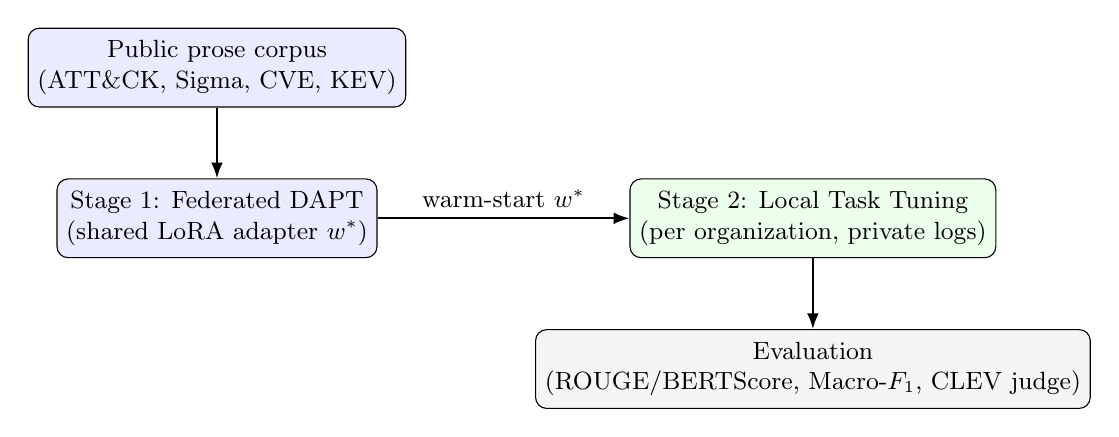
\begin{tikzpicture}[
  font=\small,
  box/.style={draw, rounded corners, align=center, minimum width=3.2cm, minimum height=1.0cm},
  arr/.style={-{Latex[length=2mm]}, thick}]
  \node[box, fill=blue!8] (corpus) {Public prose corpus\\(ATT\&CK, Sigma, CVE, KEV)};
  \node[box, fill=blue!8, below=0.9cm of corpus] (fed) {Stage 1: Federated DAPT\\(shared LoRA adapter $w^*$)};
  \node[box, fill=green!8, right=3.2cm of fed] (task) {Stage 2: Local Task Tuning\\(per organization, private logs)};
  \node[box, fill=gray!8, below=0.9cm of task] (eval) {Evaluation\\(ROUGE/BERTScore, Macro-$F_1$, CLEV judge)};
  \draw[arr] (corpus) -- (fed);
  \draw[arr] (fed) -- node[above]{warm-start $w^*$} (task);
  \draw[arr] (task) -- (eval);
\end{tikzpicture}
\caption{FeDAPT two-stage pipeline. Prose is federated (shared); logs stay local (private). Only the adapter crosses organization boundaries, and only in Stage~1.}
\label{fig:pipeline}
\end{figure}

\subsubsection{Stage 1: Federated Domain-Adaptive Pre-Training}
A network of $N$ organizations collaboratively trains a shared LoRA adapter on a curated prose corpus. Base parameters $\theta_{\text{base}}$ are frozen; LoRA parameters $w \in \mathbb{R}^d$ are updated. In each round $r \in \{1,\dots,R\}$:
\begin{enumerate}
    \item The server broadcasts the global adapter $w^{(r)}$ to all clients.
    \item Each client $i$ initializes with $w^{(r)}$ and performs $\tau$ local steps of causal language modeling on its prose shard $\mathcal{D}_i^{\text{prose}}$:
    \begin{equation}
        \mathcal{L}_{\text{DAPT}}(w) = -\sum_{t=1}^{T} \log P(x_t \mid x_{<t}; \theta_{\text{base}}, w).
    \end{equation}
    With FedProx, a proximal term constrains drift: $\mathcal{L}_{\text{FedProx}}(w) = \mathcal{L}_{\text{DAPT}}(w) + \tfrac{\mu}{2}\|w - w^{(r)}\|^2$.
    \item Clients compute $\Delta w_i = w_i^{(\tau)} - w^{(r)}$; the server aggregates to form $w^{(r+1)}$.
    \item Validation perplexity on a held-out prose set $\mathcal{D}_{\text{val}}^{\text{LM}}$ selects the best-round adapter $w^*$.
\end{enumerate}

\subsubsection{Stage 2: Local Task Tuning}
Each organization warm-starts from $w^*$ and tunes locally on its private, log-grounded dataset $\mathcal{D}_i^{\text{task}}$. We enforce \textbf{completion-only training}: prompt and padding tokens are masked with label $-100$, so loss is computed strictly over the target completion $y_{\text{target}}$:
\begin{equation}
    \mathcal{L}_{\text{task}}(w) = -\sum_{j} \log P(y_j \mid y_{<j}, x_{\text{prompt}}; \theta_{\text{base}}, w).
\end{equation}

\subsection{Data Layer and Non-IID Partitioning}
\subsubsection{Public Prose Corpus (Stage 1)}
The shared DAPT corpus is natural-language security text from four authoritative public sources: MITRE ATT\&CK Enterprise~\cite{strom2018attack} (technique, group, software, and procedure text); SigmaHQ detection-rule descriptions; NVD CVE descriptions; and the CISA Known Exploited Vulnerabilities catalog.

\subsubsection{Log Telemetry and Non-IID Dirichlet Skew (Stage 2)}
Client task data comprises raw telemetry from public, paper-backed log datasets---the AIT Log Data Set~\cite{landauer2022ait} (matched benign/attack enterprise logs), CIC-IDS2017~\cite{sharafaldin2017cicids} and UNSW-NB15~\cite{moustafa2015unsw} (network flows), and Stratus Red Team CloudTrail detonations~\cite{stratus2023}, optionally alongside \texttt{splunk/attack\_data}---each converted to a common record schema and, where applicable, supplying both the attack and benign classes from a single matched environment. \emph{These public datasets are partitioned across simulated organizations to stand in for genuinely private per-organization data.} Telemetry spans three domains: \emph{Endpoint} (Sysmon, WinEvent~4688, PowerShell), \emph{Network} (Zeek, Suricata, firewall), and \emph{Cloud} (AWS CloudTrail, Azure, Okta). To simulate enterprise heterogeneity, data is partitioned non-IID across $N{=}6$ clients using a Dirichlet distribution $\boldsymbol{p}\sim\mathrm{Dir}(\alpha)$ over domains ($\alpha{=}0.5$); small $\alpha$ concentrates domains within individual clients.

\paragraph{Label granularity (disclosure).} \texttt{attack\_data} labels are \emph{record-level}, not line-level: a telemetry record is mostly normal background activity with an attack embedded, and its technique label indicates that an attack occurred somewhere in the record. We therefore frame the verdict task at the record level---\emph{``does this activity contain evidence of attack activity?''} (labels \texttt{attack}/\texttt{benign})---rather than a per-line malicious/benign judgment the labels do not support.

\subsubsection{Task Taxonomy and Target Synthesis}
Stage~2 defines four prose-output tasks:
\begin{enumerate}
    \item \texttt{explain\_example}: case walkthrough of an attack procedure.
    \item \texttt{explain\_log}: interpretation of a raw telemetry snippet (\emph{primary}).
    \item \texttt{general\_qa}: open security-domain question answering.
    \item \texttt{verdict}: record-level attack/benign judgment with a paragraph rationale (\emph{primary}).
\end{enumerate}
Because raw logs lack natural-language targets, reference completions for the tasks are \emph{synthesized by a strong teacher LLM} (a form of distillation). Verdict negatives are drawn from the matched benign class of the same paper-backed dataset as the positives (e.g., benign AIT windows), and are only synthesized as a fallback when no matched benign source is configured. A random subset of synthesized targets is human-audited for quality; this is disclosed as a limitation (Section~\ref{sec:limitations}).

\subsection{Federated Mechanics, Privacy, and Robustness}
\subsubsection{Differential Privacy (DP-FedAvg)}
To limit membership-inference and model-inversion risk, we implement \emph{user-level} DP-FedAvg. Before aggregation, each update $\Delta w_i$ is clipped to $L_2$ bound $C$ and perturbed with Gaussian noise:
\begin{equation}
    \tilde{\Delta w}_i = \mathrm{clip}(\Delta w_i, C) + \mathcal{N}(0, \sigma^2 C^2 \mathbf{I}).
\end{equation}
Privacy loss over $R$ rounds is tracked with R\'enyi DP via an Opacus accountant for a target $\epsilon$ at $\delta{=}10^{-5}$. With full client participation each round there is no subsampling amplification; the guarantee is decentralized and round-level (not the per-example DP-SGD guarantee inside a client).

\subsubsection{Byzantine Adversary Simulations}
We model $f{=}1$ malicious client out of $N{=}6$, executing four strategies: \texttt{sign\_flip} ($\Delta w_i \to -\beta \Delta w_i$); \texttt{scale} ($\Delta w_i \to \beta \Delta w_i$, $\beta{=}10$); \texttt{gaussian} (update replaced with random noise); and \texttt{data\_poison} (input token IDs scrambled during local training). We compare \texttt{FedAvg} against \texttt{Trimmed-Mean} (coordinate-wise trimming) and \texttt{Krum} (selecting the update minimizing distance to its $n{-}f{-}2$ nearest neighbors).

\subsection{Evaluation Methodology}
Models are evaluated on held-out test splits (70/15/15 stratified). Correctness is assessed in three layers:
\begin{enumerate}
    \item \textbf{Secondary overlap metrics:} ROUGE-L and BERTScore (reported, but known to undercount semantic equivalence).
    \item \textbf{Verdict classification:} the generated verdict is parsed to a label and scored by Macro-$F_1$ against the record-level ground truth.
    \item \textbf{Primary correctness (CLEV LLM-as-a-Judge):} reference-aware binary correctness with 2+1 tie-breaking voting by independent judge models at temperature~0. The judge model differs from the model under test, and is validated against human annotations, admitted only if Cohen's $\kappa \ge 0.6$ and Macro-$F_1 \ge 0.85$.
\end{enumerate}
Configurations are selected on the validation split; the test split is reported once.

\section{Experimental Setup}
\paragraph{Model and PEFT.} Base model Mistral-7B-v0.1~\cite{jiang2023mistral} in 4-bit (NF4) QLoRA; LoRA rank $r{=}16$, $\alpha{=}32$, targeting \texttt{q\_proj}/\texttt{v\_proj}, dropout $0.05$, sequence length $512$.
\paragraph{Federated Stage 1.} $N{=}6$ clients, $R{=}20$ rounds, $\tau{=}10$ local steps, learning rate $2{\times}10^{-5}$; FedProx $\mu\in\{0,0.01\}$.
\paragraph{Privacy.} Clip $C{=}0.5$, $\delta{=}10^{-5}$, target $\epsilon \in \{1,3,8,\infty\}$ (RDP accounting).
\paragraph{Byzantine.} $f{=}1$ of $N{=}6$; scaling factor $\beta{=}10$; trimmed-mean ratio $0.2$.
\paragraph{Local Stage 2.} Learning rate $1{\times}10^{-5}$, one epoch, completion-only masking.
\paragraph{Teacher and judge models.} Reference targets are synthesized by an independent teacher LLM, and free-form correctness is scored by independent judge LLMs; both are distinct from the Mistral-7B base under test. In credit-constrained runs these are served locally (Ollama) at temperature~0---e.g., a Qwen3-14B teacher and a Gemma~3 12B $+$ Llama~3.1 8B judge panel with a third judge on disagreement---so that no metered API can rate-limit target synthesis into silent fallbacks. The exact teacher/judge models and the judge's human-validated Cohen's $\kappa$ and Macro-$F_1$ are reported alongside results.

\begin{table}[t]
\centering
\caption{Realized data pipeline (public sources; simulated federation). Prose corpus totals 35{,}033 documents.}
\label{tab:data}
\begin{tabular}{llr}
\toprule
Layer & Source / domain & Count \\
\midrule
Prose corpus & MITRE ATT\&CK & 19{,}366 \\
             & NVD CVE       & 9{,}999 \\
             & SigmaHQ       & 4{,}013 \\
             & CISA KEV      & 1{,}655 \\
\midrule
Log telemetry & Endpoint & 355 \\
              & Cloud    & 97 \\
              & Network  & 22 \\
              & General  & 101 \\
\midrule
Tasks & \texttt{explain\_log}     & 575 \\
      & \texttt{verdict} (bal.)   & 400 \\
      & \texttt{explain\_example} & 500 \\
      & \texttt{general\_qa}      & 500 \\
\bottomrule
\end{tabular}
\end{table}

\begin{figure}[t]
\centering
% produced by scripts/analyze.py (data_report/data_overview.png)
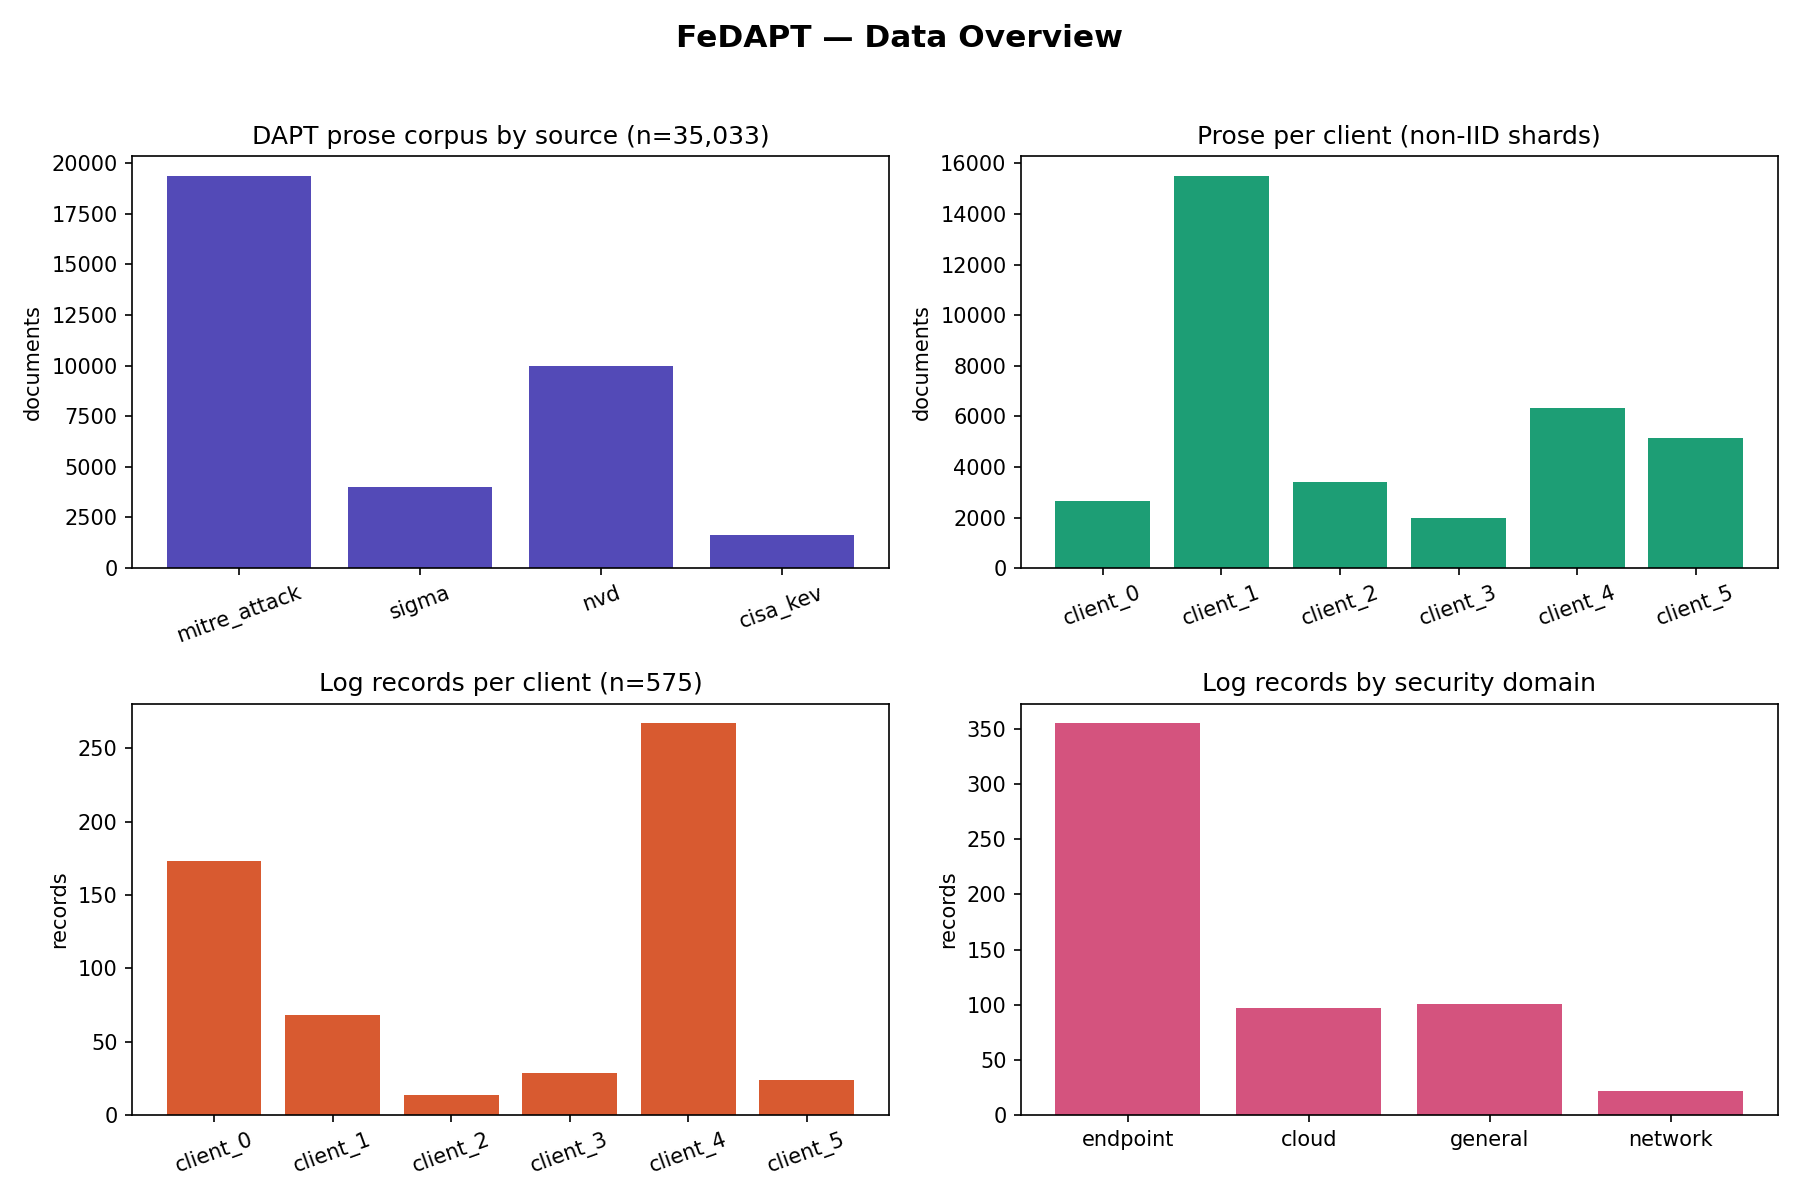
\includegraphics[width=0.95\linewidth]{data_overview.png}
\caption{Data distribution: prose corpus by source, non-IID prose shards per client, log records per client, and log records by security domain. The heavy per-client skew is the intended non-IID setting.}
\label{fig:data}
\end{figure}

\section{Experiments (Design and Expected Results)}
This section states the experimental design and the result artifacts to be reported once the full runs complete. \emph{Results tables are templates; empirical values are pending the full training matrix.}

\begin{table}[h]
\centering
\caption{Ablation over the DAPT starting point (Stage-2 tuning held fixed). $C-B$ isolates the value of federating. \emph{Values pending.}}
\label{tab:ablation}
\begin{tabular}{llccc}
\toprule
Row & Starts from & Verdict Macro-$F_1$ & CLEV correct & ROUGE-L \\
\midrule
A & No DAPT           & -- & -- & -- \\
B & Local DAPT        & -- & -- & -- \\
C & \textbf{Federated DAPT} & -- & -- & -- \\
D & Centralized DAPT  & -- & -- & -- \\
\bottomrule
\end{tabular}
\end{table}

\noindent The two headline comparisons are $C-A$ (does DAPT help at all?) and $\mathbf{C-B}$ (does \emph{federating} the DAPT beat each organization adapting alone?). We additionally report (i) a privacy--utility curve over $\epsilon \in \{1,3,8,\infty\}$, and (ii) a Byzantine comparison of FedAvg vs.\ Krum vs.\ Trimmed-Mean under each attack, expecting FedAvg to degrade while robust aggregators hold.

\section{Limitations}
\label{sec:limitations}
\begin{itemize}
    \item \textbf{Simulated federation.} Public datasets are partitioned to emulate private, per-organization data; results characterize the mechanism, not a real multi-org deployment.
    \item \textbf{Record-level labels.} \texttt{attack\_data} labels apply to whole records, not individual events, so the verdict task carries label noise; we frame and report it accordingly.
    \item \textbf{Synthesized targets.} Task references are teacher-generated (distillation); we human-audit a subset but do not exhaustively verify them.
    \item \textbf{Benign source.} We source benign negatives from the matched benign class of paper-backed datasets (e.g., AIT), keeping both classes within a single environment to avoid environment-artifact shortcuts; synthesized negatives remain a disclosed fallback when no matched source is available.
    \item \textbf{Privacy scope.} The DP guarantee is user-level, round-level, under full participation---not a per-example DP-SGD guarantee.
    \item \textbf{Scale.} The log-grounded task data is modest; conclusions on the log tasks are correspondingly preliminary.
\end{itemize}

\section{Conclusion and Future Work}
We presented FeDAPT, a two-stage federated framework that shares public security \emph{knowledge} while keeping private \emph{telemetry} local: federated domain-adaptive pre-training on prose, followed by optional local task tuning on logs. The design isolates the value of collaboration through a controlled $A/B/C/D$ ablation and stresses it under non-IID skew, differential privacy, and Byzantine adversaries, with a human-validated LLM-as-a-judge for defensible free-form scoring. Future work will complete the full experimental matrix (multiple seeds), incorporate matched-environment benign telemetry, expand the log-grounded corpus, and study additional base models and larger federations.

\begin{thebibliography}{99}
\bibitem{gururangan2020dapt} S.~Gururangan et al. Don't Stop Pretraining: Adapt Language Models to Domains and Tasks. \emph{ACL}, 2020.
\bibitem{mcmahan2017fedavg} B.~McMahan et al. Communication-Efficient Learning of Deep Networks from Decentralized Data. \emph{AISTATS}, 2017.
\bibitem{li2020fedprox} T.~Li et al. Federated Optimization in Heterogeneous Networks (FedProx). \emph{MLSys}, 2020.
\bibitem{zhang2023fedit} J.~Zhang et al. Towards Building the Federated GPT: Federated Instruction Tuning. \emph{arXiv:2305.05644}, 2023.
\bibitem{hu2021lora} E.~Hu et al. LoRA: Low-Rank Adaptation of Large Language Models. \emph{ICLR}, 2022.
\bibitem{dettmers2023qlora} T.~Dettmers et al. QLoRA: Efficient Finetuning of Quantized LLMs. \emph{NeurIPS}, 2023.
\bibitem{mcmahan2018dpfedavg} B.~McMahan et al. Learning Differentially Private Recurrent Language Models. \emph{ICLR}, 2018.
\bibitem{mironov2017rdp} I.~Mironov. R\'enyi Differential Privacy. \emph{IEEE CSF}, 2017.
\bibitem{yousefpour2021opacus} A.~Yousefpour et al. Opacus: User-Friendly Differential Privacy Library in PyTorch. \emph{arXiv:2109.12298}, 2021.
\bibitem{blanchard2017krum} P.~Blanchard et al. Machine Learning with Adversaries: Byzantine Tolerant Gradient Descent (Krum). \emph{NeurIPS}, 2017.
\bibitem{yin2018byzantine} D.~Yin et al. Byzantine-Robust Distributed Learning: Towards Optimal Statistical Rates. \emph{ICML}, 2018.
\bibitem{zheng2023judge} L.~Zheng et al. Judging LLM-as-a-Judge with MT-Bench and Chatbot Arena. \emph{NeurIPS}, 2023.
\bibitem{badshah2025clev} S.~Badshah, M.~Moustafa, H.~Sajjad. CLEV: LLM-Based Evaluation Through Lightweight Efficient Voting for Free-Form Question-Answering. \emph{arXiv:2503.08542}, 2025.
\bibitem{jiang2023mistral} A.~Jiang et al. Mistral 7B. \emph{arXiv:2310.06825}, 2023.
\bibitem{strom2018attack} B.~Strom et al. MITRE ATT\&CK: Design and Philosophy. \emph{MITRE Technical Report}, 2018.
\bibitem{landauer2022ait} M.~Landauer, F.~Skopik, M.~Frank, W.~Hotwagner, M.~Wurzenberger, A.~Rauber. Maintainable Log Datasets for Evaluation of Intrusion Detection Systems. \emph{IEEE Transactions on Dependable and Secure Computing}, 2022.
\bibitem{sharafaldin2017cicids} I.~Sharafaldin, A.~H.~Lashkari, A.~A.~Ghorbani. Toward Generating a New Intrusion Detection Dataset and Intrusion Traffic Characterization (CIC-IDS2017). \emph{ICISSP}, 2018.
\bibitem{moustafa2015unsw} N.~Moustafa, J.~Slay. UNSW-NB15: A Comprehensive Data Set for Network Intrusion Detection Systems. \emph{Military Communications and Information Systems Conference (MilCIS)}, 2015.
\bibitem{stratus2023} Datadog. Stratus Red Team: Adversary Emulation for the Cloud. Open-source tool, \url{https://github.com/DataDog/stratus-red-team}, 2023.
\bibitem{niloy2026multisource} A.~A.~Niloy, A.~Ryan, I.~H.~Rafi, M.~Erfan, M.~R.~Rahman. Multi-Source Cybersecurity Logs: An ATT\&CK-Labeled Dataset and SLM Evaluation. \emph{arXiv:2606.18190}, 2026.
\end{thebibliography}

\end{document}
